\section{Evaluation of Fides Resilience}
\label{sec:fides-resilience}

To evaluate the resilience of Fides in different scenarios, we need to find the optimal configuration for the following parameters in Fides: interaction evaluation strategy (Section~\ref{sec:interaction-evaluation-strategies}), threat intelligence aggregation function (Section~\ref{sec:network-intelligence-aggregation}) and initial reputation (Section~\ref{subsubsec:computing-reputation}). Each combination of parameters is evaluated in its capacity to correctly classify targets in \textit{any} network topology.\footnote{Distribution of correct/uncertain/incorrect/malicious peers in the network.}

In this section, we are focusing on finding the best possible combination of parameters for the worst possible scenario. In other words, we want to identify a setup, where the Fides can guarantee that it is eventually going to provide the correct data and will classify the targets correctly even though the malicious actor controls most of the network.

We shows two specific scenarios - one with no pre-trusted peers and one where there are 25\% of peers part of some pre-trusted organization. Because even the scenario with only 25\% peers shows, that in some case is Fides able to defend itself against the rest of the network, we do not show scenarios with more pre-trusted peers, but we include them in the appendix (Figure~\ref{fig:performance-all-setups-50-pretrusted}).

\subsection{Scenario With No Pre-Trusted Peers}
\label{subsec:scenario-with-0-pretrusted-peers}

In this scenario, there are no pre-trusted peers nor organizations and Fides needs to determine trust in each peer by itself.
We simulated environments starting with the 75\% of confident correct peers~(behavior from Section~\ref{subsubsec:confident-correct-peer}) up to 75\% malicious peers~(behavior from Section~\ref{subsubsec:malicious-peer}) and used all possible setups.

\cleartoleftpage % check if this appears on the left side 
\subsubsection{Target Detection Performance}

The target detection performance $tdp$ (Section~\ref{subsec:target-detection-performance-metric}) is the most important metric because it evaluates how good is Fides in the target classification - if the Fides is able to correctly come up to a conclusion that \textit{evil.com} is malicious target and \textit{google.com} is the benign.

Figure~\ref{fig:25-target-detection} visualizes the target detection performance on three different graphs where each of the graphs is a single interaction evaluation strategy.
Each graph then displays dots with different colors. Each color a single threat intelligence aggregation method in combination with different initial reputation value.
A single dot in the graph is the value of $tdp$ and in a case when the $tdp \geq 1$, it means that Fides made on average the wrong decision about the targets and classified them with the wrong label.
In other words, if $tdp \geq 1$, Fides classified benign targets as malicious and the other way around.
We included the \textit{red line} that shows $tdp = 1$ so if a dot is above the \textit{red line}, the Fides made incorrect target classification.
For that reason, we optimize the \textit{dots} to be \textit{below} the \textit{red line} (classifications being correct).

The horizontal axis in each graph measures the environment hardness explained in Section~\ref{subsec:environment-hardness}. It is important to note, that hardness essentially expresses how many peers that can provide correct data are in the simulation. For example, if the hardness is $10$, $100\%$ of peers inside the simulation are providing correct data and behave like confident correct peers.
Thus the higher the value of hardness is, the easier it is for the Fides to do correct classification.

Specifically in Figure~\ref{fig:0-target-detection} we can see that that in the \textit{easy} environment, most of \textit{dots} are below the red line until the hardness gets close to $3$.
The metrics perform more or less the same as they are able to stay bellow the red line until $eh = 3$. In that situation, the best performance and thus the lowest $tdp$ has $ThresholdTIEvaluation$ in combination with $WeighedDistanceToLocalTIEvaluation$ and initial reputation of $0.95$.

Interestingly, the $DistanceBasedTIEvaluation$ in combination with $0$ initial reputation and $AverageConfidenceTIAggregation$ for threat intelligence aggregation, shows the same target classification performance in each environment - $tdp = 0$. This suggests that the method was unable to determine any trust for any of the peers. This is then later confirmed by the Figure~\ref{fig:0-peer-trust}.

% TODO: move the legend to the left
\label{subsubsec:target-detection-performance}
\begin{figure}[hp]
    \centering
    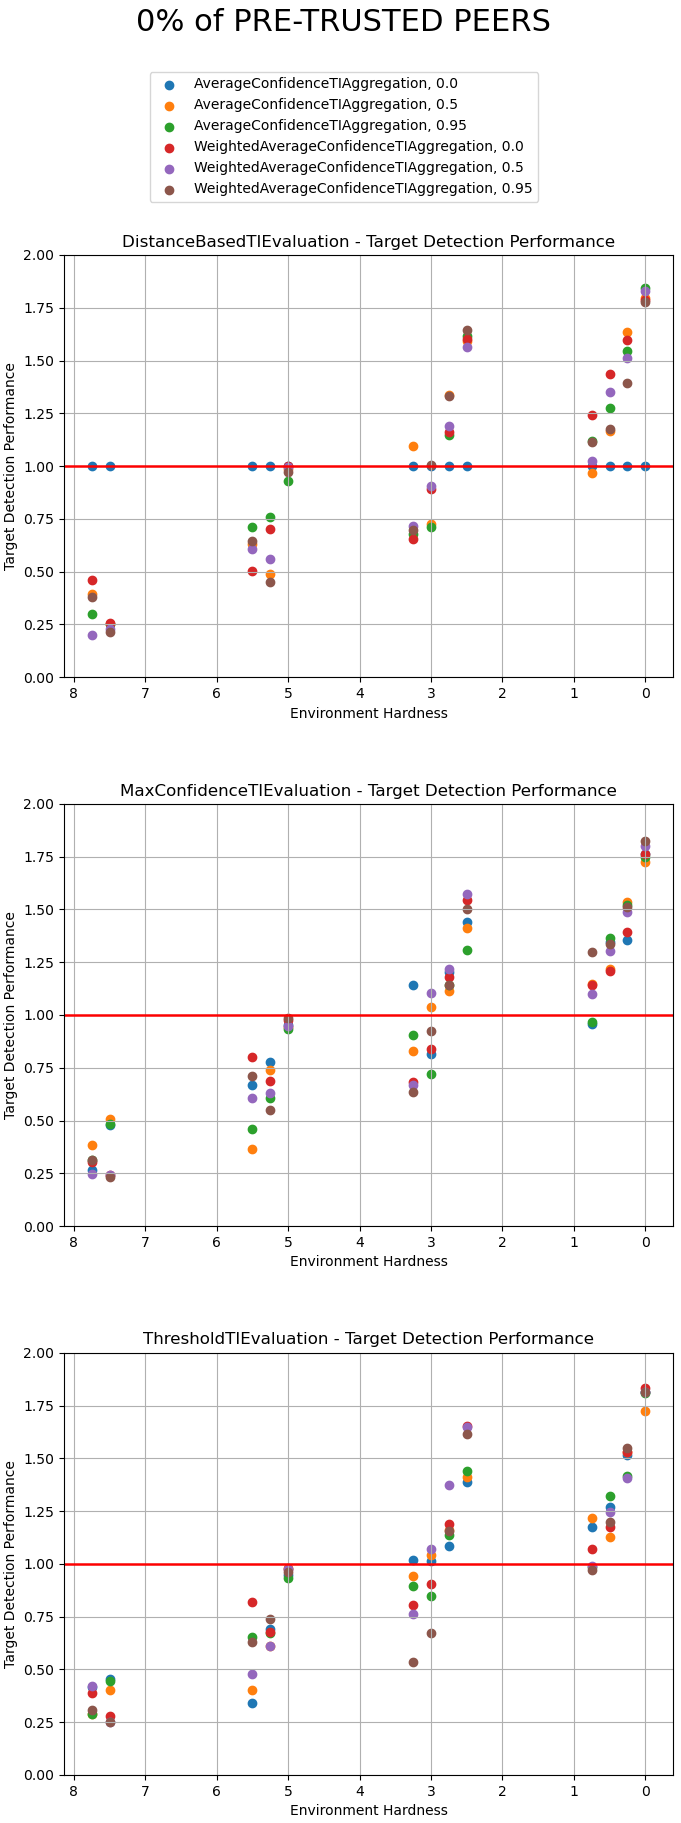
\includegraphics[height=0.95\textheight]{assets/0_target_detection.png}
    \caption{TODO}
    \label{fig:0-target-detection}
\end{figure}

\cleartoleftpage
\subsubsection{Peers Behavior Detection Performance}

\begin{figure}[hp]
    \centering
    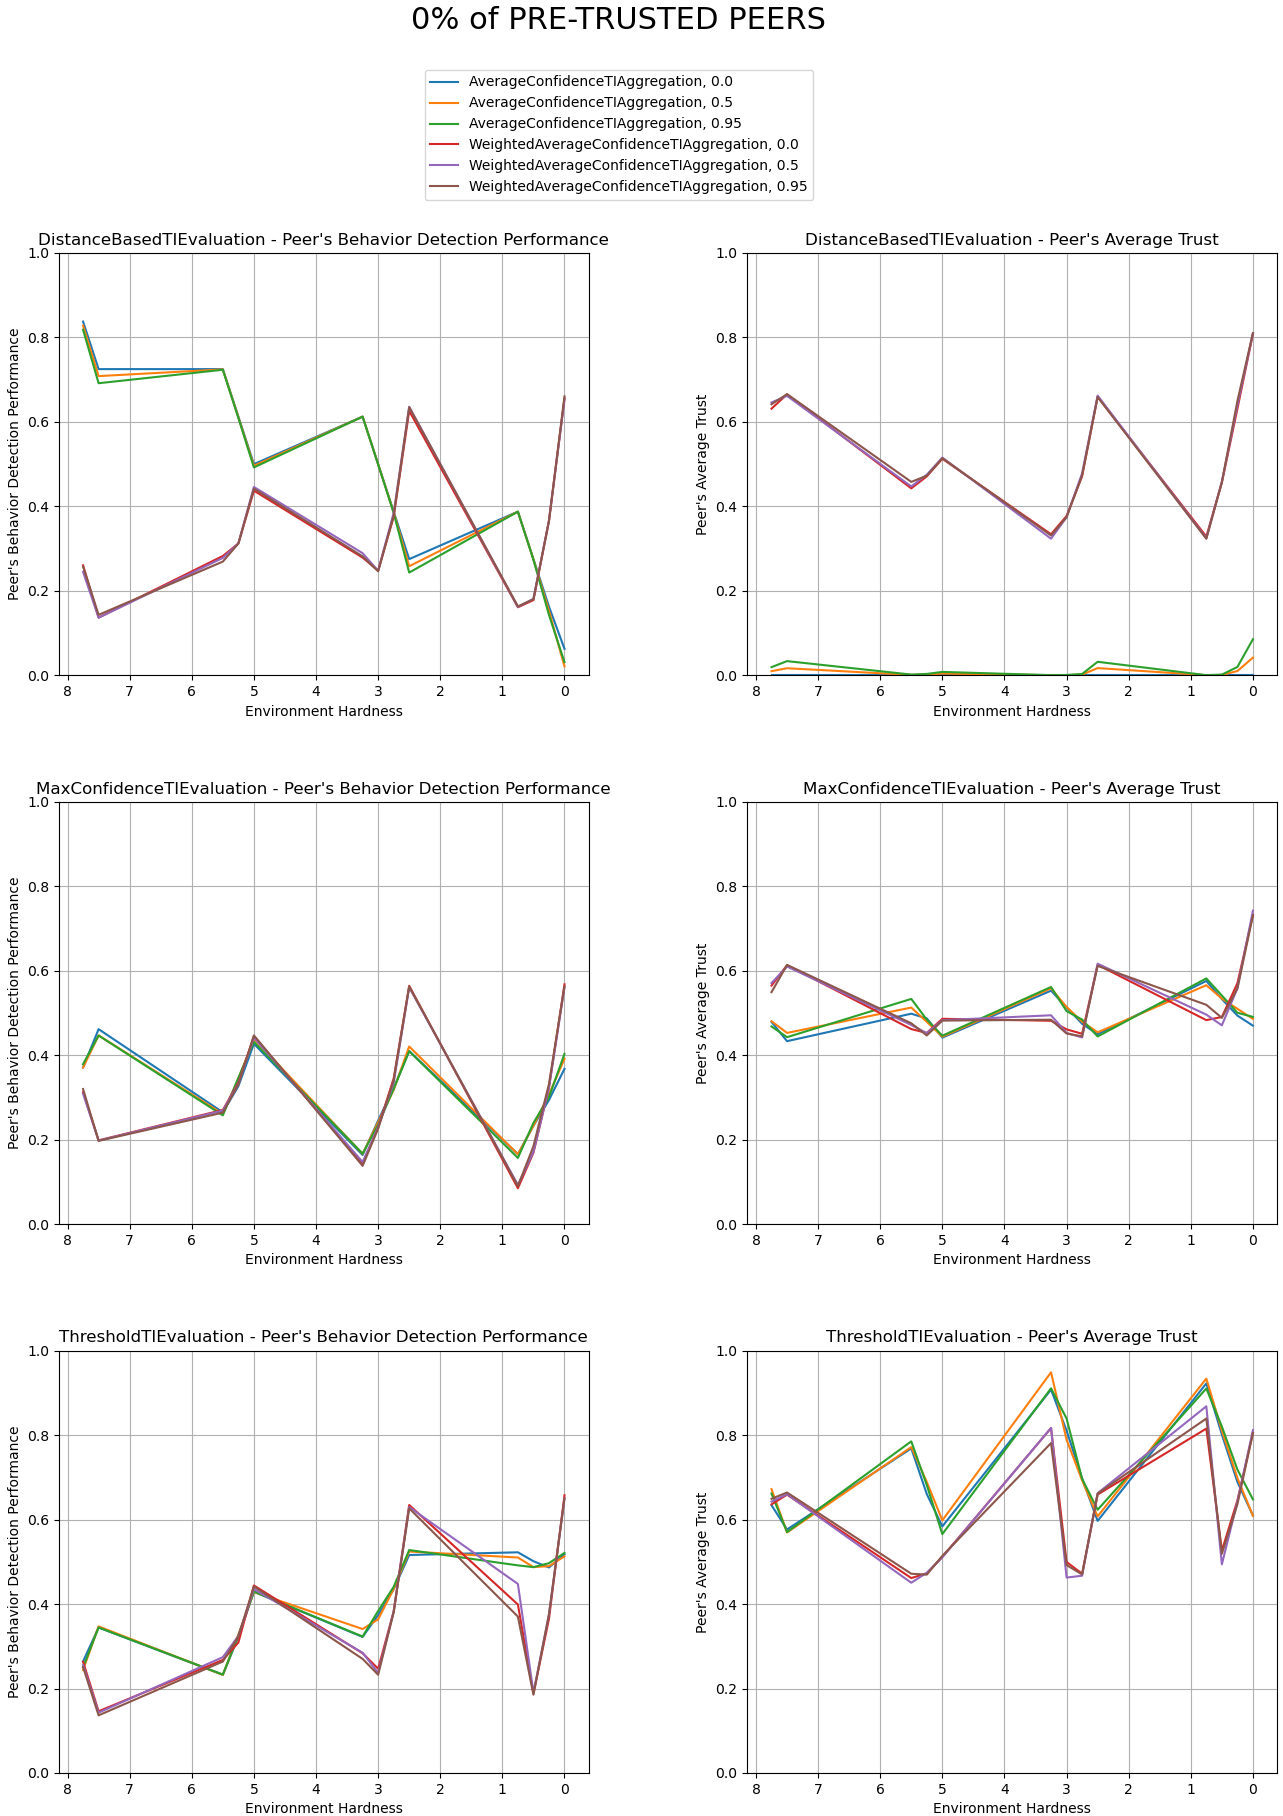
\includegraphics[width=1.0\textwidth]{assets/0_peer_trust.png}
    \caption{todo.}
    \label{fig:0-peer-trust}
\end{figure}

Figure~\ref{fig:0-peer-trust} displays two important metrics which are related to how much does Fides trust the peers in the network. First is peer's behavior detection performance metric $pbdp$ (Section~\ref{subsec:peers-behavior-detection-performance-metric}) and the second is the peer's average trust.

On the left side, one can see the peer's behavior detection performance metric that measures how good was Fides in estimating the peer's behavior. The lower value of $pbdp$ the better because the Fides's service trust for the peer was closer to the real value used in the simulation.

On the right side, we show the peer's average trust metric. That is an average trust of Fides for each peer. We include this metric in order to see how much trust was Fides able to obtain for the peers in the network.
It is important to note, that there is no \textit{correct} or \textit{desired} value of this metric, because for example in the environment where there are all peers confident correct, the peer's average trust should be high, but in the environment with all byzantine peers, this metric should be low because Fides should not trust incorrect and malicious peers.

In Figure~\ref{fig:0-peer-trust} we can see that the 

As suggested in the previous section while measuring target detection performance, the right graph for $DistanceBasedTIEvaluation$ in combination with $AverageConfidenceTIAggregation$ shows, that this setup is unable to determine trust for the peers and has average peer's trust close to $0$. This means that the trust model will almost always aggregate threat intelligence to score $0$ with confidence $0$ making it useless. 

\cleartoleftpage
\subsection{Scenario With 25\% of Pre-Trusted Peers}
\label{subsec:scenario-with-25-pretrusted-peers}

In this scenario, Fides talks to 25\% of pre-trusted peers with. We simulated environments starting with the 75\% of confident correct peers~(behavior from Section~\ref{subsubsec:confident-correct-peer}) up to 75\% malicious peers~(behavior from Section~\ref{subsubsec:malicious-peer}) and used all possible setups.

\subsubsection{Target Detection Performance}

% TODO: move the legend to the left
\label{subsubsec:target-detection-performance}
\begin{figure}[hp]
    \centering
    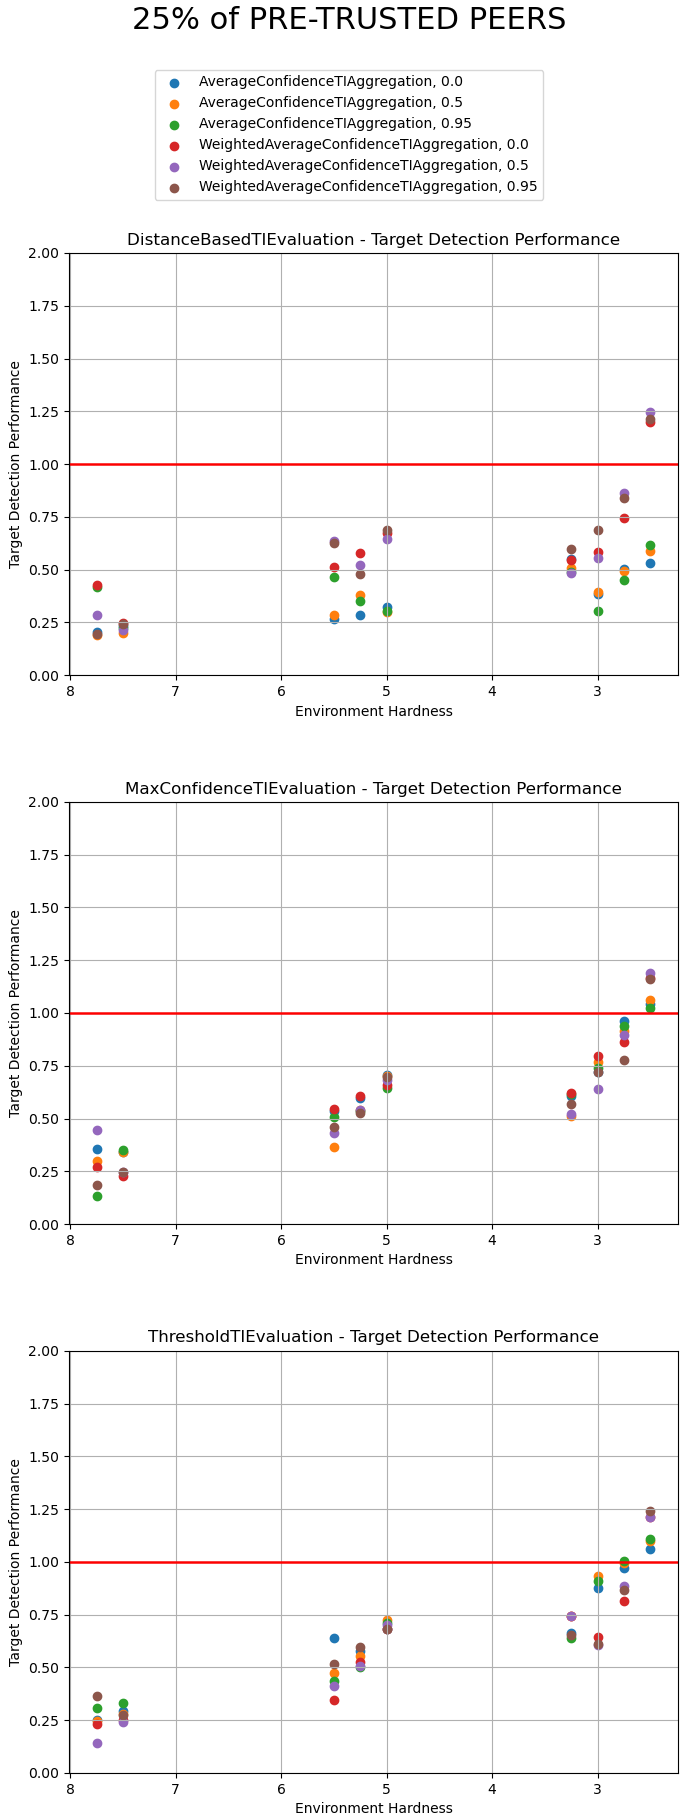
\includegraphics[height=0.95\textheight]{assets/25_target_detection.png}
    \caption{Target detection possibility.}
    \label{fig:25-target-detection}
\end{figure}

Specifically in Figure~\ref{fig:25-target-detection} one can see that until the environment hardness $eh \geq 3$, all strategies help Fides to classify targets correctly.
That changes after the environment hardness $eh \leq 2.5$ when the $ThresholdTIEvaluation$ as well as $MaxConfidenceTIEvaluation$ misclassify the targets and the $tdp \geq 1$. In that case, all threat intelligence aggregation methods are the same and all of them misclassify the targets no matter what initial reputation is used.
However, the $DistanceBasedTIEvaluation$ strategy in combination with $AverageConfidenceTIAggregation$ method is able to still classify the targets correctly and maintain the $tdp \leq 1$ even under toughest conditions where there are 75\% of adversarial peers in the simulation.

\cleartoleftpage
\subsubsection{Peers Behavior Detection Performance}

\begin{figure}[hp]
    \centering
    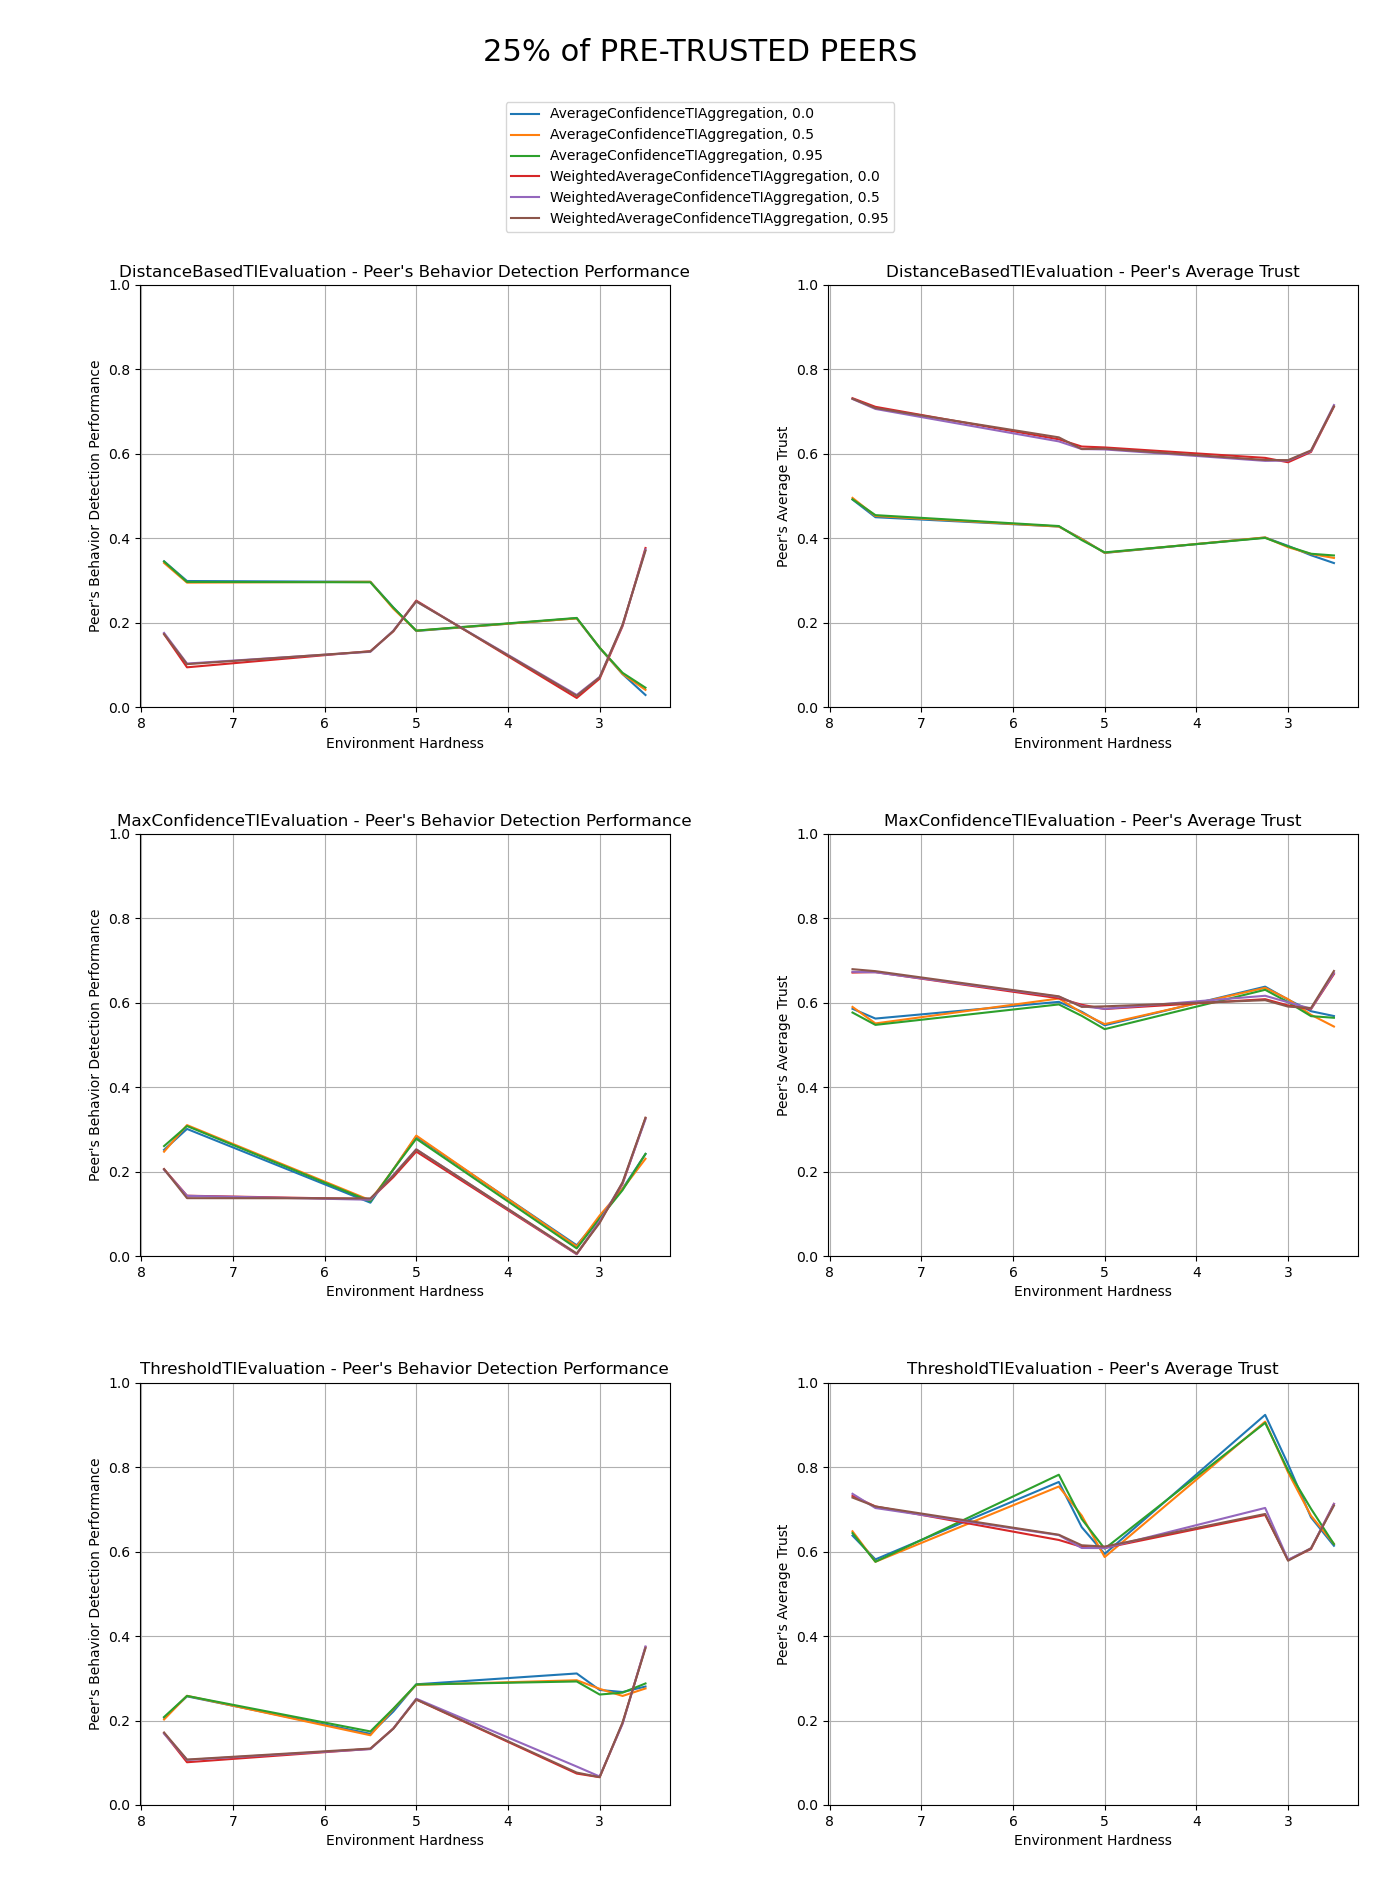
\includegraphics[width=1.0\textwidth]{assets/25_peer_trust.png}
    \caption{Target detection possibility.}
    \label{fig:25-peer-trust}
\end{figure}

TODO


% There are three rows and four columns. Each row contains a single interaction evaluation strategy (Section~\ref{sec:interaction-evaluation-strategies}) and each column contains a single metric that evaluates the behavior of that strategy in the network.
% There are three different metrics that evaluate the performance of the Fides's setup and the last graph displays how many confident correct (Section~\ref{subsubsec:confident-correct-peer}) peers there are in the network.
% The horizontal axis in each graph measures the environment hardness explained in Section~\ref{subsec:environment-hardness}.
% The vertical axis is different for each metric.

% As mentioned previously, there are three different metrics.
% The first column is a metric measuring target detection performance~(\ref{subsec:target-detection-performance-metric}), the second column is the peers' behavior detection metric~(\ref{subsec:peers-behavior-detection-performance-metric}), and the third column measures the average service trust $st^{kmax}_{i, j}$ for all peers in the simulation.

% The last, fourth, column then contains a graph that displays what percentage of peers in the simulation were confident correct~(\ref{subsubsec:confident-correct-peer}) with respect to the environment hardness value~(\ref{subsec:environment-hardness}).
% We include it in the graph to allow better visualization of how does the simulation environment looks like with respect to the peer's distribution.

% \begin{figure}[hp!]
%     \centering
%     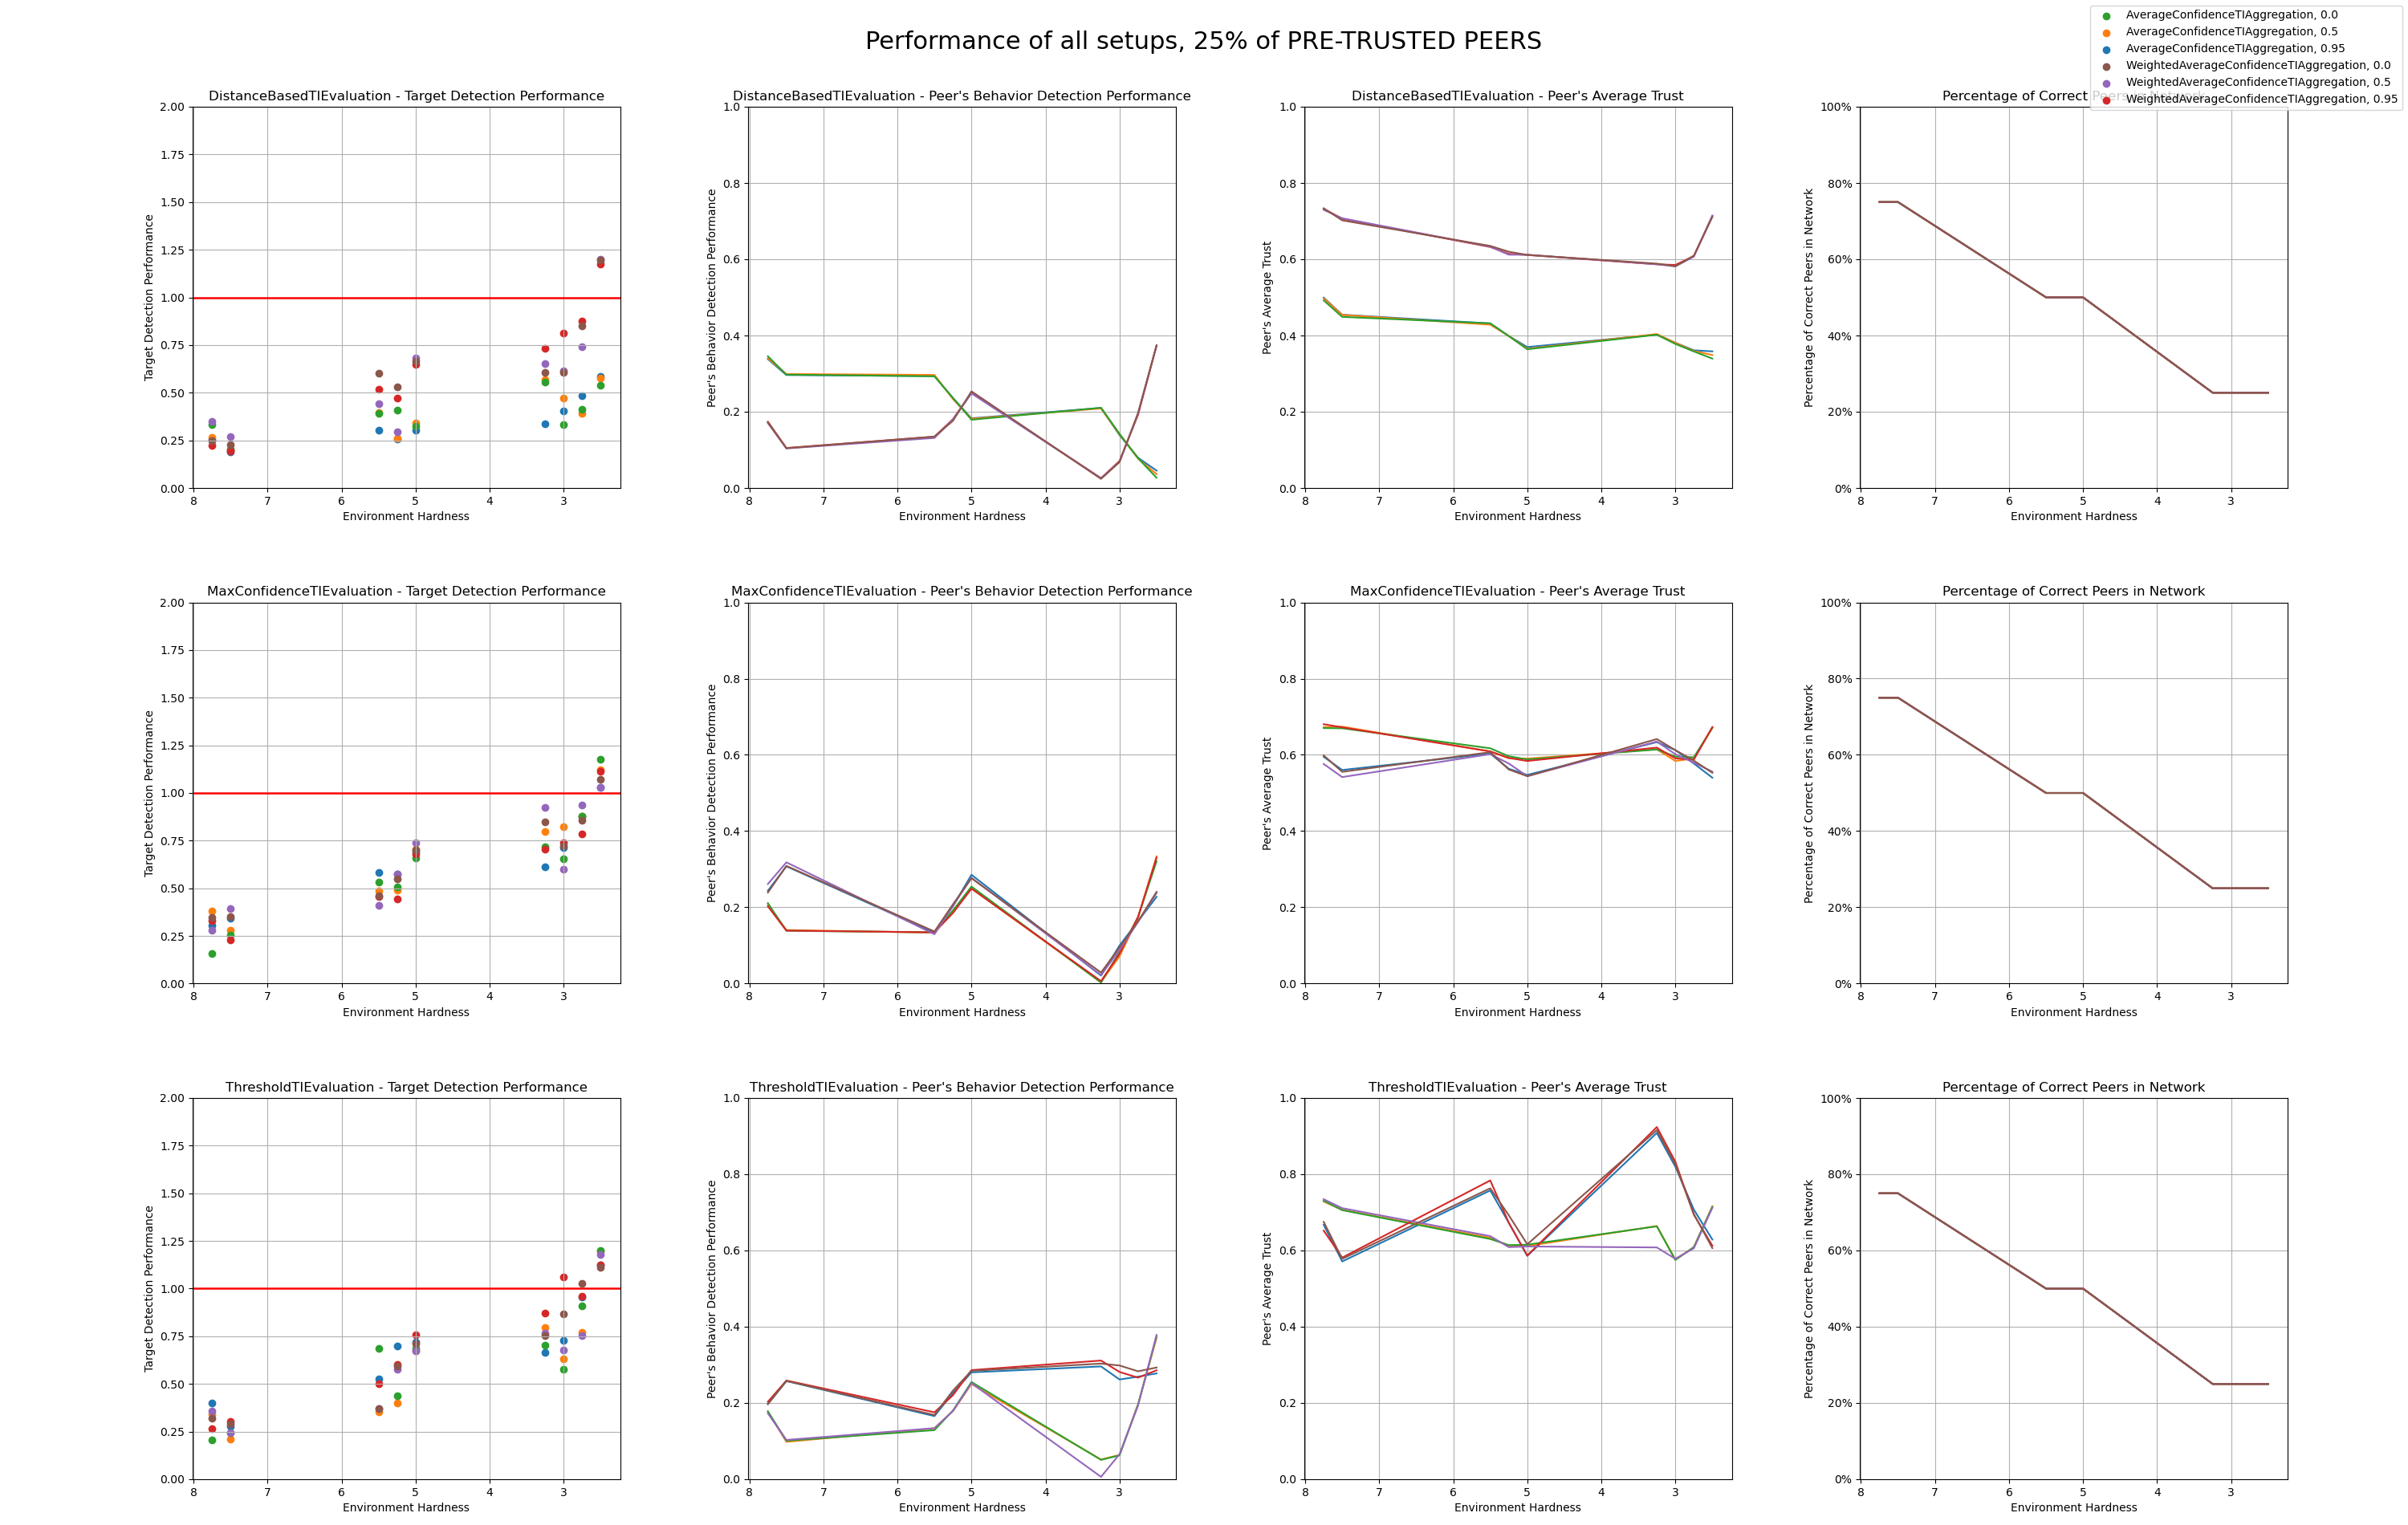
\includegraphics[width=0.94\paperwidth, angle=90]{assets/25_all_metrics.png}
%     \caption{Performance of all setups with 25\% pre-trusted peers}
%     \label{fig:performance-all-setups-25-pretrusted}
% \end{figure}

% The most important metric is the target detection performance~(\ref{subsec:target-detection-performance-metric}), which is visualized on the first graph.
% A single dot in the graph is the value of $tdp$ and in a case when the $tdp \geq 1$, it means that Fides made on average the wrong decision about the targets and classified them with the wrong label.
% In other words, if $tdp \geq 1$, Fides classified benign targets as malicious and the other way around.

% \begin{figure}[ht]
%     \centering
%     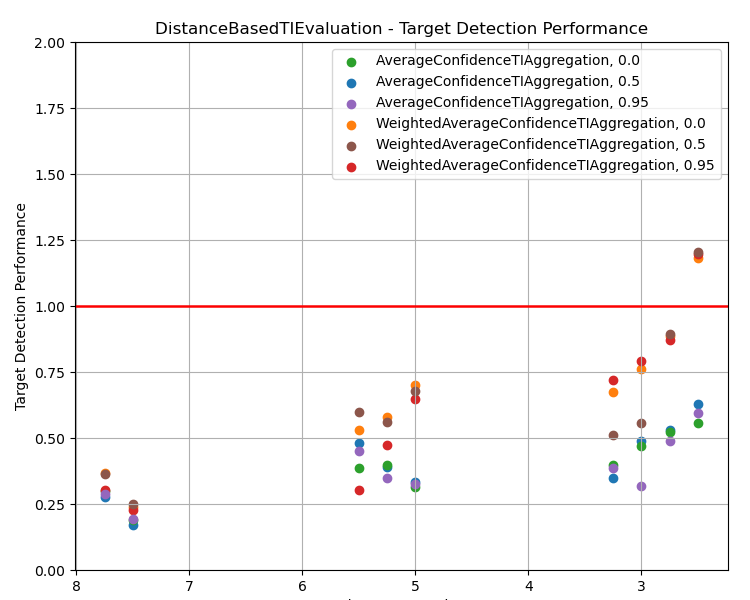
\includegraphics[width=0.7\textwidth]{assets/25_distance_detection_detail.png}
%     \caption{$DistanceBasedTIEvaluation$ with 25\% of pre-trusted peers}
%     \label{fig:distance-detection-detail-25}
% \end{figure}

% In Figure~\ref{fig:distance-detection-detail-25} we can clearly see, that there is a situation, even in the hardest environment, where the $DistanceBasedTIEvaluation$ in combination with $AverageConfidenceTIAggregation$ does not have any $tdp$ above the \textit{red line} which means that $tdp < 1$ and that Fides was always able to identify targets correctly even in the worst possible environment.

% We included the graph of this case similar to the Figure~\ref{fig:single-simulation-example} with this particular \textit{"winning"} setup in the most hostile environment to the appendix in Figure~\ref{fig:worst-best-scenario}. For the explanation of the graph see Section~\ref{sec:general-overview-of-simulation-output}.

% Interestingly, in this particular case, the initial reputation does not affect the final outcome of the simulation, but it does affect the progress as when using an initial reputation higher than $0$, Fides provides wrong scores in the situation when the malicious peers started to lie.
% However, it discovers that the peers are lying, which decreases their service trust and is able to eventually recover the correct labels for the targets.
% The score value over time for this situation can be seen on the Figure~\ref{fig:missclassification-score-only}.
% We included the whole graph in the appendix in Figure~\ref{fig:missclassification-recovery}.

% \begin{figure}[ht]
%     \centering
%     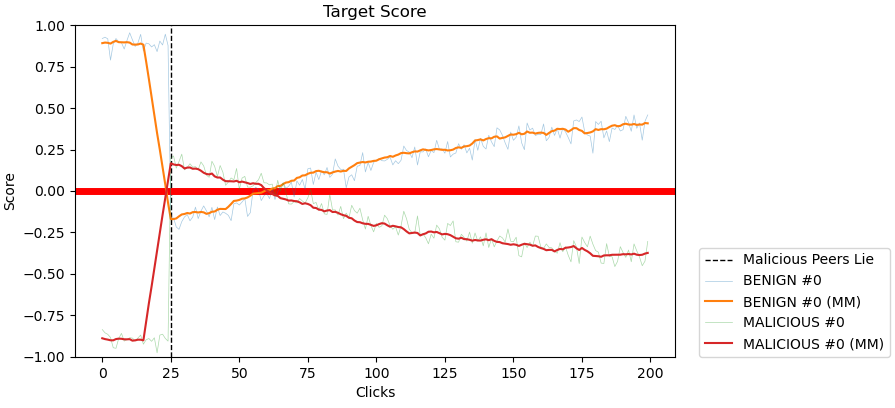
\includegraphics[width=0.9\textwidth]{assets/misclassification_score.png}
%     \caption{Score in figure~\ref{fig:missclassification-recovery}.}
%     \label{fig:missclassification-score-only}
% \end{figure}

% It is clear from Figure~\ref{fig:distance-detection-detail-25}, that when Fides used the threat intelligence aggregation method $WeightedAverageConfidenceTIAggregation$~(\ref{subsec:WeightedAverageConfidenceTIAggregation}), it miss-classified the targets in one situation.
% Thus, this method does not provide a guarantee that Fides will end up with correct classifications for every target.

% The same applies to all other interaction evaluation methods as we can see in the Figure~\ref{fig:performance-all-setups-25-pretrusted} that in the hardest environment, they all classified the targets poorly with all threat intelligence aggregation methods.

% \subsection{Scenarios of No pre-trusted peers, and 50\% pre-trusted peers}
% \label{subsec:resilience-under-different-conditions}
% Other two important scenarios to consider are the situations where the administrator does not have any pre-trusted peers and when at least 50\% of peers are pre-trusted.

% With no pre-trusted peers in the network, the results of each configuration vary and they highly depend on the network topology as well as on the knowledge of the local Slips instance. The results for the no pre-trusted scenario are shown in Appendix Figure~\ref{fig:performance-all-setups-0-pretrusted}.


% In the scenario of 50\% pre-trusted peers, no matter the configuration, Fides was eventually able to determine the correct target classification with a high precision of $tdp \leq 0.7$. Moreover, Fides was able to correctly identify the peer's behavior with the precision of $pbdp \leq 0.2$. This is a very favorable situation for the administrator, where you trust the peers so much that it is not possible for the adversarial peers to modify the belief. The results for this scenario are shown in Appendix Figure~\ref{fig:performance-all-setups-50-pretrusted}.

% \subsection{Discussion}
% We discovered that actually there \textbf{exists} a particular setup that guarantees that Fides is able to eventually classify the targets correctly in a very adversarial situation. When Fides communicates with at least 25\% of pre-trusted peers from pre-trusted organizations ($0.25 \cdot |P|$ are pre-trusted) and uses $DistanceBasedTIEvaluation$ (section~\ref{subsec:distance-based-eval}) for evaluating the interactions in combination with $AverageConfidenceTIAggregation$ (Section~\ref{subsec:AverageConfidenceTIAggregation}) for aggregating the threat intelligence; then Fides is able to correctly classify the targets no matter how many adversarial peers are in the network (up to filling the remaining 75\%) or how hard they lie.
